\documentclass[resume]{subfiles}



\begin{document}
\section{C++}
\subsection{friend}
\begin{lstlisting}[style=Cpp]
class A {
private:
	// La classe B peut accéder aux méthodes privées de A
	friend class B;
	// La fonction calc de C peut accédéer aux méthodes privées de A
	friend int C::calc(int x);
	// La fonction main peut accédéer aux méthodes privées de A (à éviter)
	friend int main();
}
\end{lstlisting}
\subsection{Polymorphisme}
\subsubsection{static binding}
\begin{lstlisting}[style=Cpp]
class A {
public:
	void display() { cout << "A" << endl;};
};
class B : public A {
public:
	void display() {cout << "B" << endl;};
};

int main() {
	A a;
	B b;
	A* p;
	p = &a;
	p->display(); -> "A"
	p = &b;
	p->display(); -> "A"
}
\end{lstlisting}
\subsubsection{Dynamic binding}
\begin{lstlisting}[style=Cpp]
class A {
public:
	virtual void display() { cout << "A" << endl;};
};
class B : public A {
public:
	virtual void display() {cout << "B" << endl;};
};

int main() {
	A a;
	B b;
	A* p;
	p = &a;
	p->display(); -> "A"
	p = &b;
	p->display(); -> "B"
}
\end{lstlisting}
\subsubsection{Interfaces}
\begin{lstlisting}[style=Cpp]
class IVehicle {
public:
	virtual void drive() = 0;
};
class Car : public IVehicle {
public:
	virtual void drive() { cout << "car drives" << endl;}
};
class Rocket : public IVehicle {
public:
	virtual void drive() { cout << "rocket flies" << endl;}
};
int main() {
	IVehicle* v1 = new Rocket();
	IVehicle* v2 = new Car();
	v1->drive(); // car
	v2->drive(); // rocket
	delete v1;
	delete v2;
};
\end{lstlisting}
\subsection{Classes génériques}
\begin{lstlisting}[style=Cpp]
vector<T> vInt(5);
\end{lstlisting}
\subsection{UML}
\begin{figure}[H]
\centering
\includegraphics[width=7cm,page=3]{Schemas-crop.pdf}
\end{figure}
\begin{figure}[H]
\centering
\includegraphics[width=7cm,page=2]{Schemas-crop.pdf}
\end{figure}

\subsubsection{Diagrammes de classe}
\begin{figure}[H]
\centering
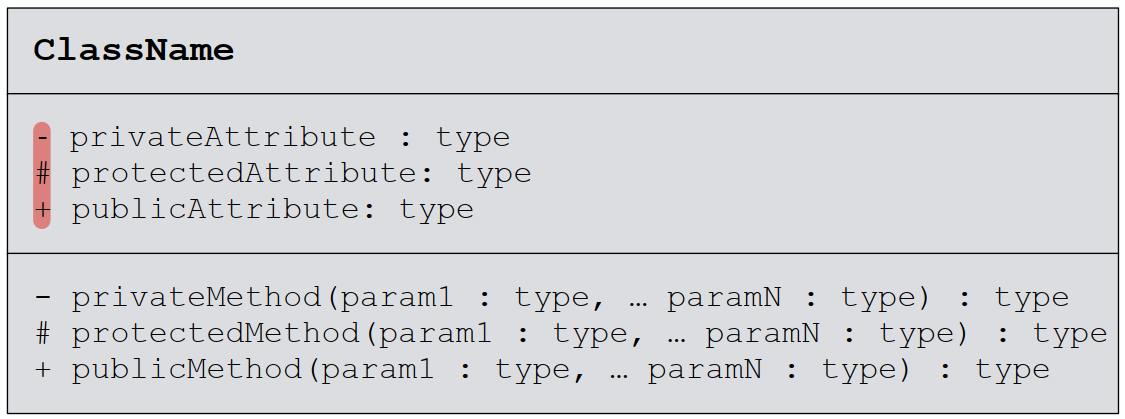
\includegraphics[width=7cm]{Figures/UML/diagClass.png}
\end{figure}

\subsubsection{Diagrammes de séquences}
\begin{figure}[H]
\centering
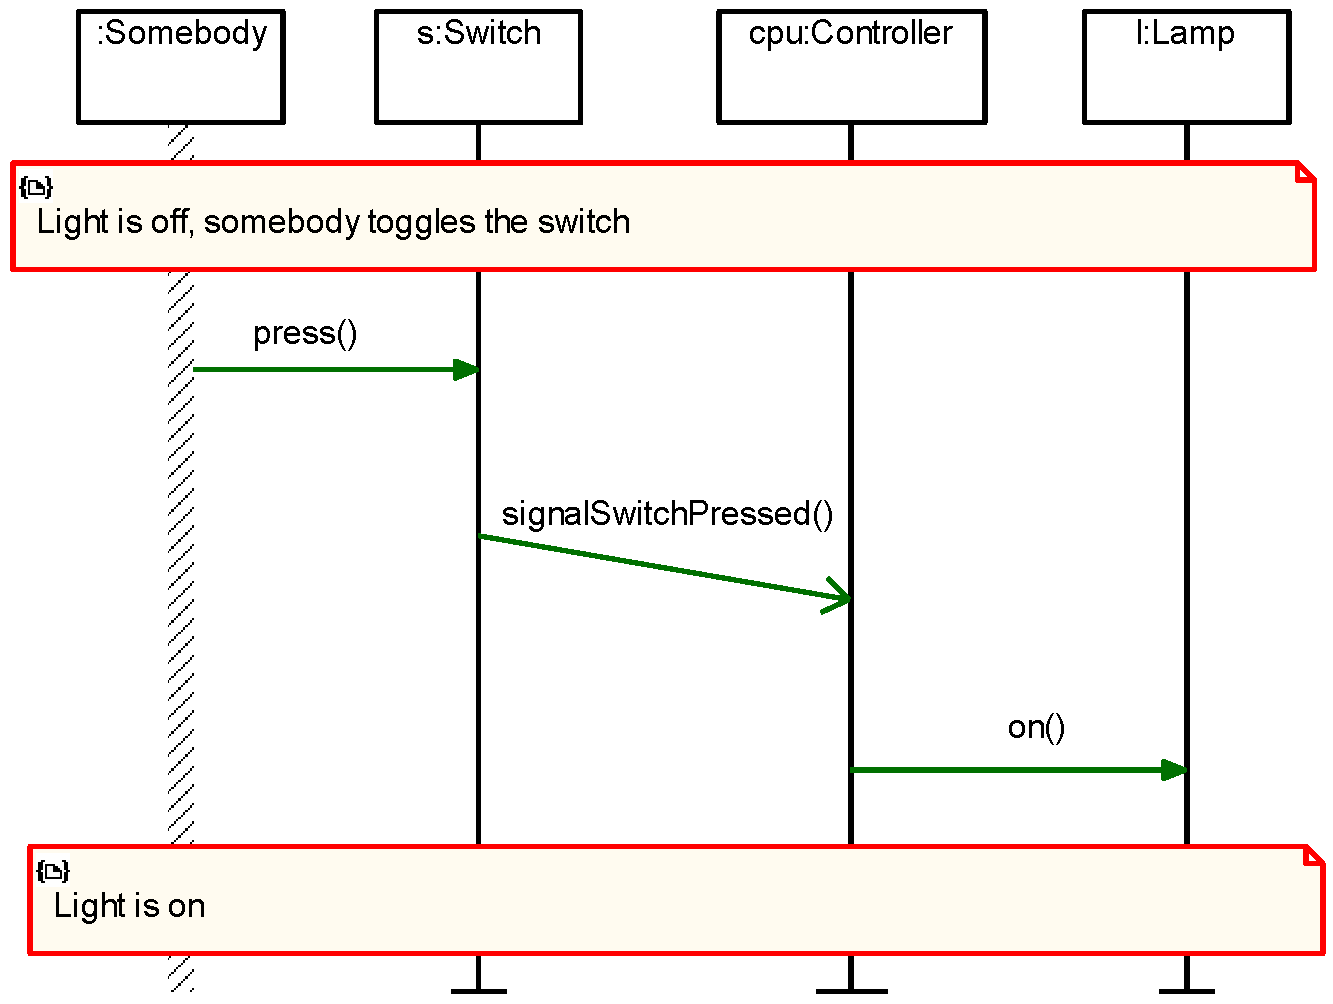
\includegraphics[width=7cm]{img_0.pdf}
\end{figure}

\subsubsection{Diagrammes d'états}
\begin{figure}[H]
\centering
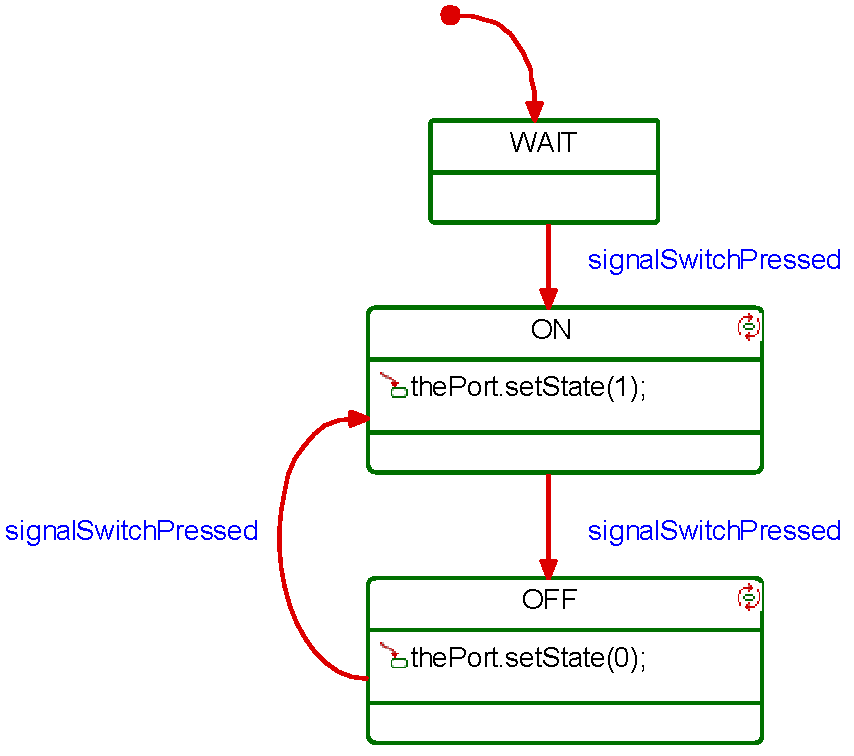
\includegraphics[width=5cm]{img_1.pdf}\\
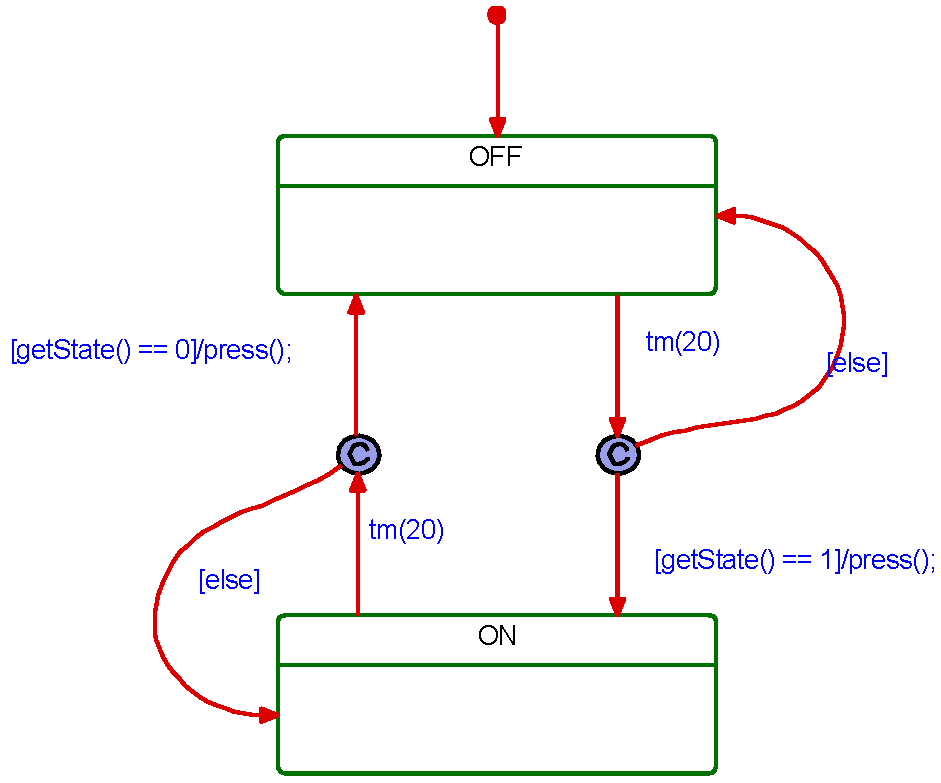
\includegraphics[width=5cm]{img_2.pdf}
\end{figure}

\subsection{Singleton}
\begin{lstlisting}[style=Cpp]
class Singleton {
public:
	static Singleton& getInstance() {
		static Singleton instance;
		return instance;
	}
private:
	// Private constructor and desctructor
	Singleton() {};
	Singleton(const Singleton&) {};
	void operator=(const Singleton&) {};
};

int main() {
	Singleton::getInstace().doSomething();
}
\end{lstlisting}






\end{document}